\documentclass{beamer}
\usetheme{Warsaw}

\usepackage[utf8]{inputenc}
\usepackage{fancybox}
\usepackage{multimedia} 
\usepackage{subfig}
\usepackage{amsmath}
\usepackage{hyperref}
\usepackage{marvosym}

\usepackage[all]{xy}
\begin{document}


\title[Digitale Bildverarbeitung] % (optional, only for long titles)
{Digitale Bildverarbeitung
\\
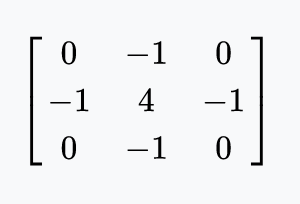
\includegraphics[scale=1.0]{img/cover}
}
\subtitle{}
\author[Dr. Johannes Riesterer] % (optional, for multiple authors)
{Dr.  rer. nat. Johannes Riesterer}

\date[KPT 2004] % (optional)
{}

\subject{Digitale Bildverarbeitung}

\frame{\titlepage}


\begin{frame}
    \frametitle{Kantenerkennung}
\framesubtitle{}
\begin{block}{Kanten}
Kanten sind durch schnelle Änderungen des Farbwertes gekennzeichnet. Sie sind damit Extremstellen der ersten Ableitung.
\end{block}
\begin{figure}[htp]
      \centering
Intensität und Gradient entlang eines Bildschnittes \\
    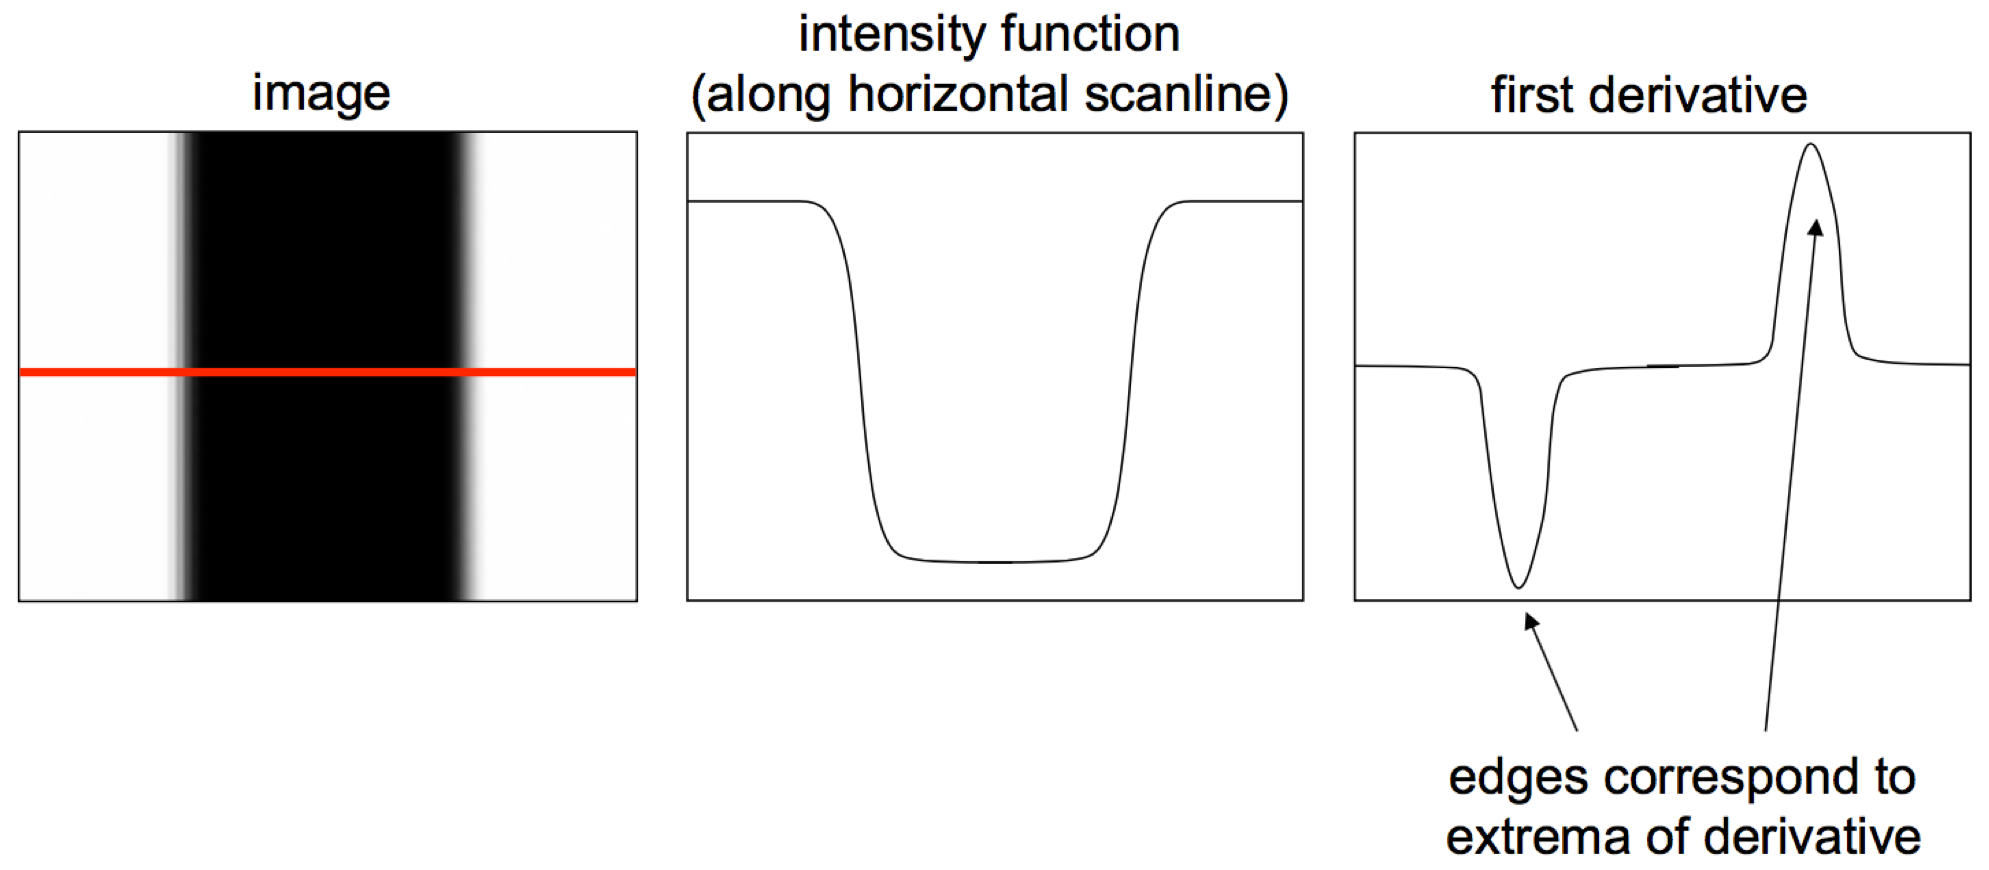
\includegraphics[width=0.65\textwidth]{img/edgedetection} 
      \caption{Quelle: ai.stanford.edu}
\end{figure}

 \end{frame}

\begin{frame}
    \frametitle{Kantenerkennung}
\framesubtitle{}
\begin{block}{Gradientenbasierte Kantenerkennung}
Bei der Detektion von Kanten mit Hilfe des Gradienten ist   Rauschen ein Problem, da sich  hier ebenfalls  der Farbwert schnell ändert. 
\end{block}
\begin{figure}[htp]
      \centering
Rauschen \\
    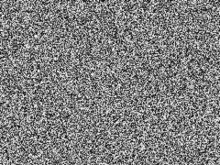
\includegraphics[width=0.45\textwidth]{img/noise} 
      \caption{Quelle: Wikipedia}
\end{figure}

 \end{frame}

\begin{frame}
    \frametitle{Kantenerkennung}
\framesubtitle{}
\begin{block}{Gradientenbasierte Kantenerkennung}
Idee: Wende einen Filter an, der das Rauschen reduziert und bilde dann den Gradienten. Bilde also den Gradienten
\begin{align*}
\frac{\partial (u * f)(x)}{\partial x} 
\end{align*}
wobei $f$ ein Faltungskern ist.
\end{block}

\begin{block}{Ableitung von Faltungen}
Es gilt
\begin{align*}
\frac{\partial (u * f)(x)}{\partial x} = (u * f')(x)
\end{align*}

\end{block}

 \end{frame}


\begin{frame}
    \frametitle{Kantenerkennung}
\framesubtitle{}
\begin{block}{Gradientenbasierte Kantenerkennung}
Welcher Filter ist gut geeignet?
\end{block}
\begin{block}{Kantenerkennung nach Canny}
Es gibt Kanten auf unterschiedlichen Skalen ("grobe Kanten" und "feine Kanten"). Wähle daher einen parameterabhängigen Faltungskern
$f_\sigma$. Zu einem Originalbild $u_0$ bekommen wir eine ganze Klasse von Bildern
\begin{align*}
u(x, \sigma) = u_0 * f_\sigma(x) \;.
\end{align*}
 \end{block}

 \end{frame}

\begin{frame}
    \frametitle{Kantenerkennung}
\framesubtitle{}

\begin{block}{Kantenerkennung nach Canny}
Die Stellen der Kanten soll sich bei wachsendem $\sigma$ nicht verändern und ebenso sollen auch keine Kanten hinzukommen. 
Deswegen soll in einem Kantenpunkt $x_0$ von $u_0$ gelten:
\begin{align*}
\frac{\partial^2}{\partial x^2} > 0 \Rightarrow \frac{\partial}{\partial \sigma}  u(x_0, \sigma) > 0 \\
\frac{\partial^2}{\partial x^2} = 0 \Rightarrow \frac{\partial}{\partial \sigma}  u(x_0, \sigma) = 0 \\
\frac{\partial^2}{\partial x^2} < 0 \Rightarrow \frac{\partial}{\partial \sigma}  u(x_0, \sigma) <0
\end{align*}
 \end{block}

 \end{frame}

\begin{frame}
    \frametitle{Kantenerkennung}
\framesubtitle{}

\begin{block}{Kantenerkennung nach Canny}
Für einen allgemeinen Punkt soll daher gelten:
\begin{align*}
&\frac{\partial^2}{\partial x^2}  u(x, \sigma)  =  \ \frac{\partial}{\partial \sigma}  u(x, \sigma)  \\
&  u(x, 0) = u_0(x) 
\end{align*}
 \end{block}

\begin{block}{Kantenerkennung nach Canny}
Diese partielle Differentialgleichung hat die eindeutige Lösung
\begin{align*}
&  u(x, \sigma) = (u_0 * G^{\sqrt{2\sigma}}) (x)
\end{align*}
wobei $ G^{\sqrt{2\sigma}}$ der Gaußfilter ist.
 \end{block}

 \end{frame}


\begin{frame}
    \frametitle{Kantenerkennung}
\framesubtitle{}

\begin{block}{Kantenerkennung nach Canny}
Die Kantenerkennung nach Canny faltet ein gegebenes Bild $u$ zuerst mit einem Gaußkernel $G^{\sigma}$. Danach wird  der Betrag der Ableitung und seine Richtung berechnet: 
\begin{align*}
p(x) = & || \nabla (u * G^\sigma)(x) || \\
&= \sqrt{ (\frac{\partial}{\partial x_1} (u * G^\sigma)(x))^2 + (\frac{\partial}{\partial x_2} (u * G^\sigma)(x))^2 } \\
\theta(x) & = \angle  \nabla (u * G^\sigma)(x) = \arctan \biggl( \frac{\frac{\partial}{\partial x_2} (u * G^\sigma)(x)}{\frac{\partial}{\partial x_1} (u * G^\sigma)(x)} \biggr)
\end{align*}


 \end{block}

 \end{frame}



\begin{frame}
    \frametitle{Kantenerkennung}
\framesubtitle{}
\begin{block}{Kantenerkennung nach Canny}
Als Kanten werden lokale Maxima von $p(x)$ in Richtung $(\sin \theta(x), \cos \theta(x)  )$
\end{block}
\begin{figure}[htp]
      \centering
Kanten als lokale Maxima in Kantenrichtung \\
    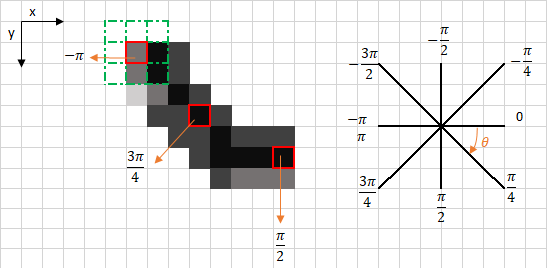
\includegraphics[width=0.55\textwidth]{img/canny_max} 
      \caption{Quelle: towardsdatascience.com}
\end{figure}

 \end{frame}




\begin{frame}
    \frametitle{Kantenerkennung}
\framesubtitle{}
\begin{block}{Kantenschärfen mit Laplace}
Durch die Operation $u - \tau \bigtriangleup u$ werden die Kanten hervorgehoben.
\end{block}
\begin{figure}[htp]
      \centering
Kanten als lokale Maxima in Kantenrichtung \\
    \includegraphics[width=0.55\textwidth]{img/laplace1} \\
    \includegraphics[width=0.35\textwidth]{img/laplace2} 
      \caption{Quelle:OpenCV}
\end{figure}
 \end{frame}

\begin{frame}
    \frametitle{Kantenerkennung}
\framesubtitle{}
\begin{figure}[htp]
      \centering
Kantenschärfung \\
    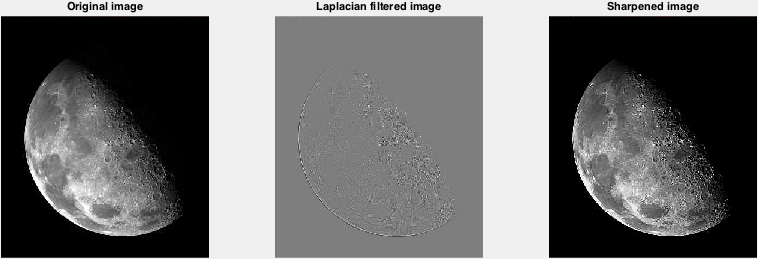
\includegraphics[width=0.95\textwidth]{img/sharpening} 
      \caption{Quelle: Stackoverflow}
\end{figure}
 \end{frame}



\begin{frame}
    \frametitle{Segmentierung}
\framesubtitle{}
\begin{block}{Segmentierung}
 Die Erzeugung von inhaltlich zusammenhängenden Regionen durch Zusammenfassung benachbarter Pixel oder Voxel entsprechend einem bestimmten Homogenitätskriterium bezeichnet man als Segmentierung. 
\end{block}
\begin{block}{Segmentierung}
Szene $\to$ Bildaufnahme  $\to$ Bildvorverarbeitung  $\to$ Segmentierung  $\to$ Merkmalsextraktion  $\to$ Klassifizierung  $\to$ Aussage 
\end{block}
 
\end{frame}



\begin{frame}
    \frametitle{Segmentierung}
\framesubtitle{}
\begin{block}{Segmentierung}

\begin{figure}[htp]
      \centering
Schwellwert \\
    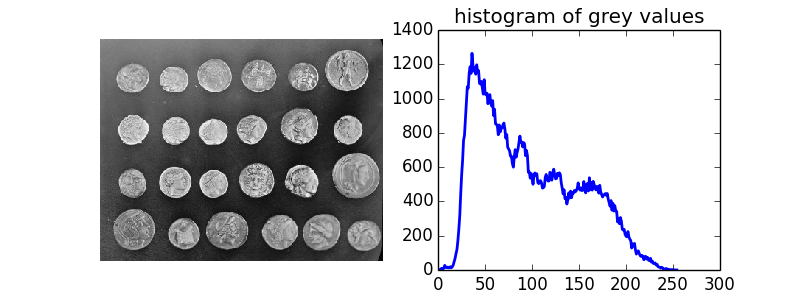
\includegraphics[width=0.95\textwidth]{img/segmentation_edge1} 
      \caption{Quelle: scikit-image.org}
\end{figure}
\end{block}

 \end{frame}




\begin{frame}
    \frametitle{Segmentierung}
\framesubtitle{}
\begin{block}{Segmentierung über Intensität-Schwellwert}

\begin{figure}[htp]
      \centering
Schwellwert \\
    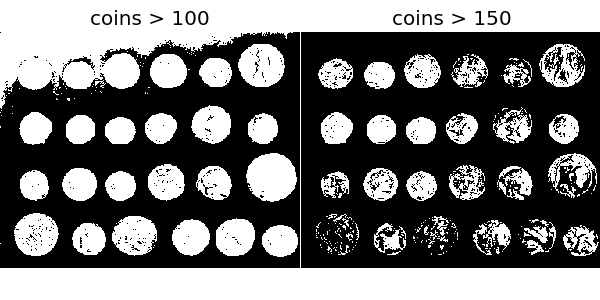
\includegraphics[width=0.95\textwidth]{img/segmentation_thresh1} 
      \caption{Quelle: scikit-image.org}
\end{figure}
\end{block}

 \end{frame}


\begin{frame}
    \frametitle{Segmentierung}
\framesubtitle{}
\begin{block}{Kantenbasierte Segmentierung }
1. Kantenerkennung nach Canny
\end{block}
\begin{figure}[htp]
      \centering
Canny \\
    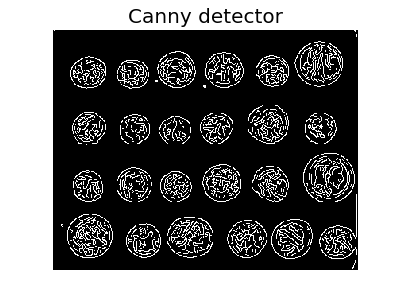
\includegraphics[width=0.55\textwidth]{img/segmentation_edge2} 
      \caption{Quelle: scikit-image.org}
\end{figure}


 \end{frame}



\begin{frame}
    \frametitle{Segmentierung}
\framesubtitle{}
\begin{block}{Kantenbasierte Segmentierung }
2. Löcher Füllen mit morphologischem Filter
\end{block}
\begin{figure}[htp]
      \centering
Canny + morphologischem Filter \\
    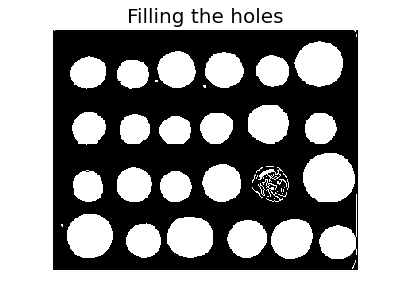
\includegraphics[width=0.55\textwidth]{img/segmentation_edge3} 
      \caption{Quelle: scikit-image.org}
\end{figure}


 \end{frame}

\begin{frame}
    \frametitle{Segmentierung}
\framesubtitle{}
\begin{block}{Kantenbasierte Segmentierung }
3. Kleine Objekte entfernen mit morphologischem Filter
\end{block}
\begin{figure}[htp]
      \centering
Canny + morphologischem Filter  + morphologischem Filter  \\
    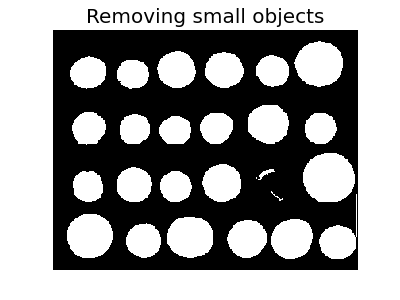
\includegraphics[width=0.55\textwidth]{img/segmentation_edge4} 
      \caption{Quelle: scikit-image.org}
\end{figure}


 \end{frame}


\begin{frame}
    \frametitle{Segmentierung}
\framesubtitle{}
\begin{block}{Segmentierung über K-Means}
Ziel von ''k''-Means ist es, den Datensatz so in ''k'' Partitionen zu teilen, dass die Summe der quadrierten Abweichungen von den Cluster-Schwerpunkten minimal ist. Mathematisch entspricht dies der Optimierung der Funktion
\begin{align*}
J = \sum_{i=1}^{k}  \sum_{\mathbf x_j \in S_{i}} {\| \mathbf x_j - \boldsymbol \mu_i \|^2}
\end{align*}
mit den Datenpunkten $ \mathbf x_j $  und den Schwerpunkten$ \boldsymbol \mu_i$ der Cluster $S_i$.

\end{block}


 \end{frame}



\begin{frame}
    \frametitle{Segmentierung}
\framesubtitle{}
\begin{block}{Segmentierung über K-Means}
\begin{itemize}
 \item Initialisierung: Wähle $k$ zufällige Mittelwerte (''Means''): $ \mathbf m_1^{(1)}, \ldots, \mathbf m_k^{(1)} $ aus dem Datensatz.
 \item  Zuordnung: Jedes Datenobjekt wird demjenigen Cluster zugeordnet, bei dem die Cluster-Varianz am wenigsten erhöht wird. 
\begin{align*}
S_i^{(t)} = \left\{ \mathbf x_j : \big\| \mathbf x_j - \mathbf m^{(t)}_i \big\|^2 \leq \big\| \mathbf x_j - \mathbf m^{(t)}_{i^*} \big\|^2 \text{ für alle }i^*=1,\ldots,k \right\} 
\end{align*}
\item Aktualisieren: Berechne die Mittelpunkte der Cluster neu 
\begin{align*}
\mathbf m_i^{(t+1)} = \frac{1}{|S_i^{(t)}|} \sum_{\mathbf x_j \in S_{i}^{(t)}} \mathbf x_j  
\end{align*}
\end{itemize}
\end{block}


 \end{frame}





\begin{frame}
    \frametitle{Segmentierung}
\framesubtitle{}
\begin{figure}[htp]
      \centering
Segmentierung des Farbraumes über K-Means \\
    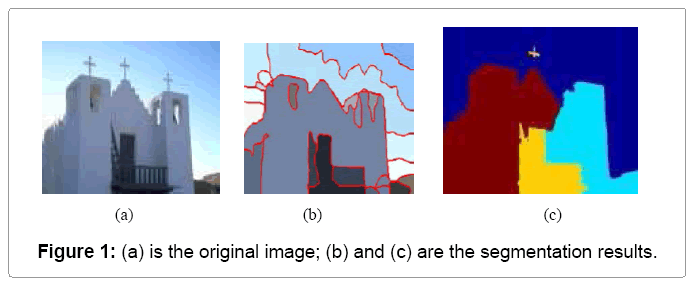
\includegraphics[width=0.85\textwidth]{img/segmentation_kmeans} 
      \caption{Quelle:towardsdatascience.com}
\end{figure}


 \end{frame}


\begin{frame}
    \frametitle{Segmentierung}
\framesubtitle{}
\begin{block}{Segmentierung über K-Means}
Ist die Anzahl der Clusterzentren unbekannt, kann man den Algorithmus mit verschiedenen Anzahlen von Zentren $k$ ausführen und die 
Fehler miteinander vergleichen. Es gibt meistens einen Punkt, ab dem sich der Fehler nicht mehr signifikant ändert. Diesen kann man zum Beispiel wählen.
(Elbowmethod). 
\end{block}

\begin{figure}[htp]
      \centering
Elbow Method \\
    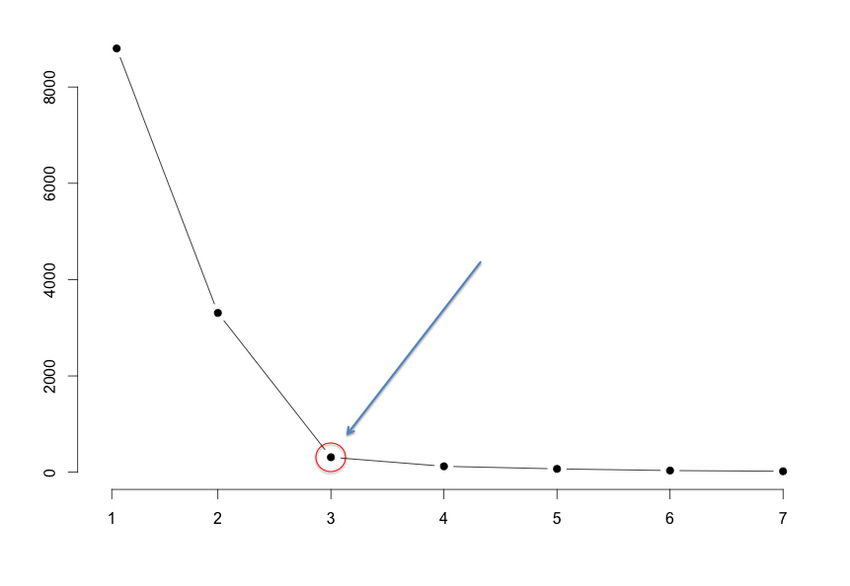
\includegraphics[width=0.45\textwidth]{img/kmeans_elbow} 
      \caption{Quelle:  mubaris.com}
\end{figure}

 \end{frame}

\end{document}
